\section{طراحی و پیاده‌سازی سامانه پیشنهادی}

\subsection{مقدمه}

پس از تعیین چارچوب کلی پژوهش و انتخاب معیار مرجع برای ارزیابی عملکرد بیماران، گام بعدی طراحی سامانه‌ای بود که بتواند تمامی مراحل مورد نیاز از ثبت داده‌های حرکتی تا پیش‌بینی نمرات عملکردی را پوشش دهد. از آنجا که هدف این پژوهش صرفاً بررسی یک الگوریتم یادگیری ماشین نبود، توسعه سامانه به گونه‌ای انجام شد که تمامی مراحل اندازه‌گیری، مدیریت داده‌ها، پردازش سیگنال و تحلیل اطلاعات به صورت یک فرآیند منسجم در کنار یکدیگر قرار گیرند.

فرآیند توسعه سامانه به صورت مرحله‌ای انجام شد. در ابتدا زیرساخت سخت‌افزاری برای ثبت داده‌های حرکتی طراحی گردید. پس از آن، نرم‌افزار لازم برای دریافت، نمایش و ذخیره‌سازی داده‌های حسگرها توسعه داده شد تا امکان ایجاد یک بانک اطلاعاتی منظم از آزمون‌های انجام‌شده فراهم شود. در ادامه، داده‌های ثبت‌شده وارد مرحله پیش‌پردازش شدند و پس از استخراج ویژگی‌های مناسب، مدل‌های مختلف یادگیری ماشین برای پیش‌بینی نمرات عملکردی آموزش داده شدند.

با توجه به ماهیت میان‌رشته‌ای پروژه، توسعه سامانه را می‌توان در سه بخش اصلی خلاصه کرد:

\begin{itemize}
	\item طراحی و پیاده‌سازی سامانه اندازه‌گیری مبتنی بر حسگرهای اینرسیایی؛
	\item توسعه ابزارهای نرم‌افزاری برای دریافت، مدیریت و پردازش داده‌ها؛
	\item طراحی و ارزیابی مدل‌های یادگیری ماشین برای پیش‌بینی نمرات عملکردی.
\end{itemize}

در ادامه این فصل، ابتدا معماری کلی سامانه معرفی می‌شود و سپس جزئیات هر یک از بخش‌های سخت‌افزاری و نرم‌افزاری، فرآیند ثبت داده‌ها، مراحل پردازش اطلاعات و طراحی مدل‌های یادگیری ماشین به تفصیل تشریح خواهد شد.

\subsection{روند انتخاب روش ارزیابی در پژوهش حاضر}

پس از تعریف کلی مسئله پژوهش، نخستین گام بررسی روش‌های متداول ارزیابی عملکرد حرکتی بیماران مبتلا به دیستروفی عضلانی دوشن بود. هدف از این مرحله، انتخاب روشی بود که علاوه بر اعتبار بالینی، امکان اندازه‌گیری آن با استفاده از حسگرهای اینرسیایی نیز وجود داشته باشد.

در ابتدا، طی جلساتی با تیم پزشکی همکار، فرآیند متداول ارزیابی بیماران مبتلا به دیستروفی عضلانی دوشن معرفی شد. در این جلسات علاوه بر مرور روش‌های رایج ارزیابی، تجربیات حاصل از پروژه‌های پیشین نیز مطرح شد. یکی از این تجربیات مربوط به استفاده از حسگرهای الکترومایوگرافی سطحی
\footnote{\lr{Surface Electromyography (sEMG)}}
برای تحلیل وضعیت بیماران بود. اگرچه این روش اطلاعات ارزشمندی از فعالیت عضلات فراهم می‌کرد، اما پیچیدگی نصب حسگرها، حساسیت زیاد سیگنال‌ها به شرایط ثبت و دشواری استخراج شاخص‌های پایدار موجب شده بود که استفاده از آن برای اهداف این پروژه مناسب ارزیابی نشود. این تجربه، استفاده از حسگرهای اینرسیایی را به عنوان گزینه اصلی ثبت حرکت در پژوهش حاضر مطرح کرد.

در ادامه، تعدادی از آزمون‌های متداول ارزیابی عملکرد بیماران از جمله آزمون شش دقیقه راه رفتن (\lr{Six-Minute Walk Test}) و برخی مقیاس‌های عملکردی دیگر مورد مطالعه قرار گرفتند. هرچند این آزمون‌ها اطلاعات مفیدی درباره وضعیت کلی بیمار ارائه می‌کنند، اما بررسی آن‌ها نشان داد که بسیاری از شاخص‌های حاصل از این آزمون‌ها به صورت مستقیم با داده‌های قابل استخراج از حسگرهای اینرسیایی قابل ارتباط نیستند و یا تنها بخشی از توانایی‌های حرکتی بیمار را ارزیابی می‌کنند.

به منظور شناخت بهتر فرآیند ارزیابی بالینی، در ادامه این پژوهش، جلسات معاینه بیماران در مرکز درمانی مورد مشاهده قرار گرفت. در این جلسات، پزشک متخصص با استفاده از آزمون‌های عملکردی مختلف، توانایی بیماران در انجام فعالیت‌هایی نظیر راه رفتن، برخاستن از صندلی، نشستن، برخاستن از روی زمین، بالا رفتن از پله و سایر حرکات عملکردی را بررسی می‌کرد. همچنین در برخی آزمون‌ها، قدرت عضلانی بیمار از طریق اعمال نیرو توسط پزشک یا درخواست اعمال نیرو از سوی بیمار ارزیابی می‌شد. مشاهده مستقیم این فرآیند نقش مهمی در شناخت معیارهای مورد توجه پزشک هنگام ارزیابی عملکرد بیماران داشت.

پس از مطالعه روش‌های مختلف و بررسی امکان پیاده‌سازی آن‌ها با استفاده از حسگرهای اینرسیایی، مقیاس‌های عملکردی دیگری از جمله \lr{Motor Function Measure (MFM)} نیز مورد بررسی قرار گرفتند. با این حال، تحلیل ساختار این آزمون‌ها نشان داد که بخش قابل توجهی از آیتم‌های آن‌ها نیازمند ارزیابی‌هایی هستند که تنها از طریق داده‌های حرکتی ثبت‌شده توسط \lr{IMU} قابل اندازه‌گیری نیستند یا به تجهیزات مکمل نیاز دارند.

در نهایت، با جمع‌بندی مطالعات انجام‌شده، مشاهدات بالینی و بررسی قابلیت اندازه‌گیری حرکات مختلف توسط حسگرهای اینرسیایی، مقیاس \lr{North Star Ambulatory Assessment (NSAA)} به عنوان معیار مرجع این پژوهش انتخاب شد. این مقیاس علاوه بر برخورداری از اعتبار بالینی در ارزیابی بیماران مبتلا به \lr{DMD}، شامل مجموعه‌ای از فعالیت‌های عملکردی است که بخش قابل توجهی از آن‌ها قابلیت تحلیل از طریق داده‌های سینماتیکی ثبت‌شده توسط حسگرهای اینرسیایی را دارند.

مطالعات ارزیابی پایایی و روایی این ابزار نشان داده‌اند که \lr{NSAA} از اعتبار بالایی برای پایش تغییرات عملکردی بیماران دیستروفی عضلانی دوشن برخوردار است، با این حال وابستگی آن به مشاهده مستقیم و قضاوت ارزیاب می‌تواند منجر به تغییرپذیری بین‌ارزیاب شود \cite{Mayhew2013Reliability}. این موضوع به‌ویژه در مواردی که تمایز بین اجرای «طبیعی» و اجرای «اصلاح‌شده» ظریف است، اهمیت بیشتری پیدا می‌کند.

از منظر مهندسی تحلیل حرکت، بسیاری از معیارهای کیفی
\lr{NSAA}
(مانند استفاده از حرکات جبرانی، تغییر در دامنه حرکتی یا کاهش سرعت اجرای حرکت) می‌توانند با تغییر در پارامترهای سینماتیکی قابل‌اندازه‌گیری همراه باشند. بنابراین، کمی‌سازی این شاخص‌ها با استفاده از حسگرهای پوشیدنی می‌تواند به توسعه یک چارچوب داده‌محور مکمل برای فرآیند نمره‌دهی کمک نماید. از این رو، 
\lr{NSAA}
 به عنوان مبنای طراحی سامانه پیشنهادی و برچسب‌گذاری داده‌های این پژوهش مورد استفاده قرار گرفت.

\begin{figure}[H]
	\centering
	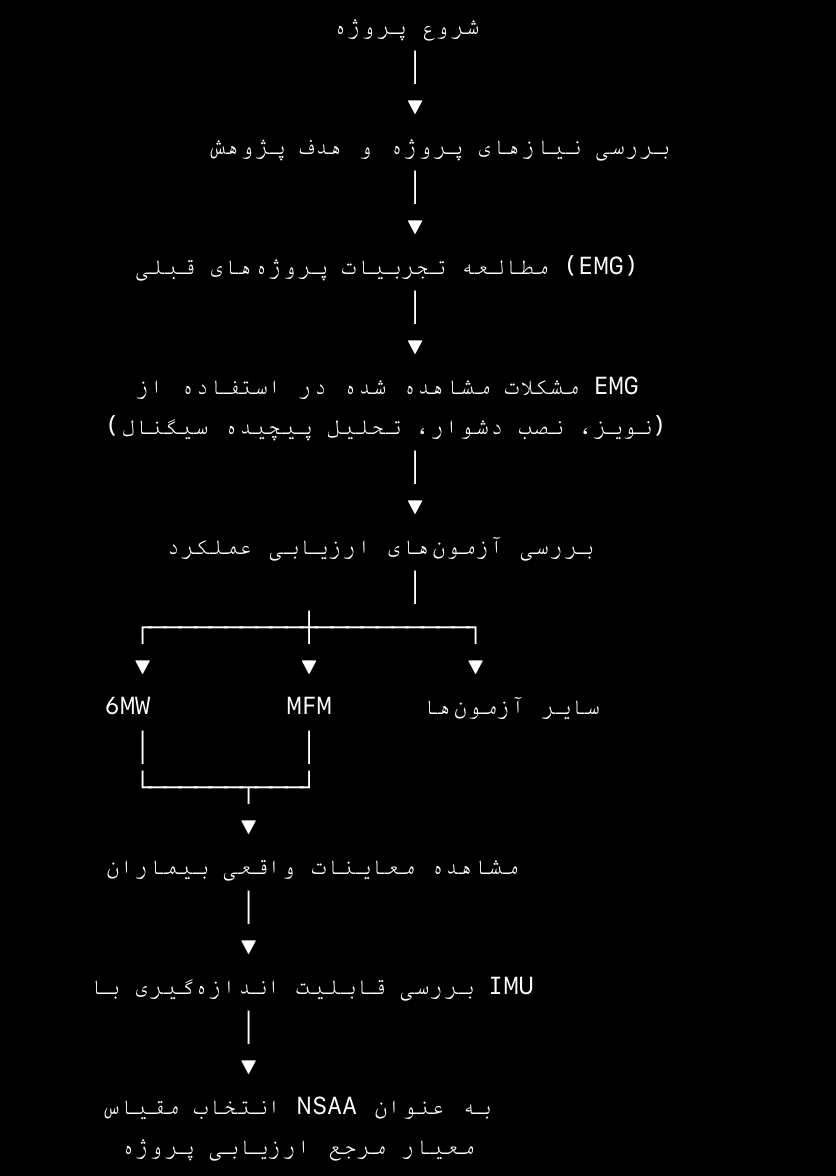
\includegraphics[width=0.4\linewidth]{Images/1_FlowChartChoosingNSAA}
	\caption{روند تصمیم‌گیری برای انتخاب روش ارزیابی عملکرد}
	\label{fig:1flowchartchoosingnsaa}
\end{figure}


\subsection{انتخاب مقیاس \lr{NSAA} به عنوان معیار ارزیابی}

پس از بررسی روش‌های مختلف ارزیابی عملکرد حرکتی و مطالعه قابلیت اندازه‌گیری آن‌ها با استفاده از حسگرهای اینرسیایی، لازم بود یک معیار استاندارد به عنوان مرجع نمره‌دهی در این پژوهش انتخاب شود. این معیار علاوه بر اعتبار بالینی، باید شامل فعالیت‌هایی باشد که بتوان آن‌ها را به کمک داده‌های سینماتیکی ثبت‌شده توسط حسگرهای اینرسیایی تحلیل کرد.

در این راستا، مقیاس \lr{North Star Ambulatory Assessment (NSAA)} به عنوان یکی از معتبرترین ابزارهای ارزیابی عملکرد بیماران سرپایی مبتلا به دیستروفی عضلانی دوشن مورد بررسی قرار گرفت. این مقیاس به طور اختصاصی برای بیماران \lr{DMD} طراحی شده و امروزه در بسیاری از مراکز درمانی و مطالعات بالینی به عنوان یکی از معیارهای اصلی پایش روند پیشرفت بیماری مورد استفاده قرار می‌گیرد \cite{Scott2009NSAA,Mayhew2013Reliability}.

\lr{NSAA} شامل ۱۷ فعالیت عملکردی است که بخش عمده‌ای از توانایی‌های حرکتی بیماران را پوشش می‌دهد. فعالیت‌هایی مانند برخاستن از صندلی، برخاستن از روی زمین، راه رفتن، بالا رفتن از پله، ایستادن روی یک پا، پریدن و دویدن، از جمله آیتم‌های این مقیاس هستند. هر فعالیت بر اساس کیفیت اجرای حرکت در یکی از سه سطح عملکردی امتیازدهی می‌شود که به ترتیب بیانگر ناتوانی در انجام حرکت، انجام حرکت همراه با الگوهای جبرانی و انجام طبیعی حرکت است.

یکی از مهم‌ترین دلایل انتخاب \lr{NSAA} در این پژوهش، همخوانی قابل توجه بسیاری از آیتم‌های آن با قابلیت‌های حسگرهای اینرسیایی بود. در اغلب این فعالیت‌ها، اطلاعاتی مانند شتاب، سرعت زاویه‌ای، مدت زمان انجام حرکت و الگوی کلی حرکت می‌توانند شاخص‌هایی کمی از کیفیت اجرای فعالیت در اختیار قرار دهند. بنابراین انتظار می‌رود بتوان بخشی از قضاوت بالینی پزشک را با استفاده از تحلیل داده‌های ثبت‌شده توسط حسگرها مدل‌سازی کرد.

بر همین اساس، در پژوهش حاضر \lr{NSAA} به عنوان معیار مرجع برای برچسب‌گذاری داده‌ها و ارزیابی عملکرد مدل‌های یادگیری ماشین انتخاب شد. در ادامه گزارش، نحوه ثبت داده‌ها، استخراج ویژگی‌ها و طراحی مدل‌های پیش‌بینی بر مبنای این مقیاس به تفصیل تشریح خواهد شد.



\subsection{انتخاب حسگرهای اینرسیایی برای ثبت حرکات}

پس از انتخاب چارچوب مناسب برای ارزیابی عملکرد بیماران، گام بعدی انتخاب ابزاری بود که بتواند اطلاعات مورد نیاز از حرکات بیماران را ثبت کند. در سال‌های اخیر فناوری حسگرهای پوشیدنی پیشرفت چشمگیری داشته و ابزارهای متعددی برای اندازه‌گیری حرکت انسان توسعه یافته‌اند. در میان این ابزارها، حسگرهای اینرسیایی (\lr{Inertial Measurement Unit - IMU}) به دلیل ابعاد کوچک، هزینه پایین و امکان استفاده در محیط‌های خارج از آزمایشگاه، توجه بسیاری از پژوهشگران را به خود جلب کرده‌اند \cite{MuroDeLaHerran2014Wearable}.

در سال‌های اخیر، استفاده از حسگر اینرسیایی در تحلیل حرکت انسان به‌طور گسترده‌ای افزایش یافته است، زیرا این حسگرها نسبت به سیستم‌های موشن‌کپچر اپتیکال دارای مزایایی نظیر هزینه کمتر، قابلیت حمل، عدم وابستگی به شرایط نوری و امکان استفاده در محیط‌های غیرآزمایشگاهی هستند \cite{MuroDeLaHerran2014Wearable}. این ویژگی‌ها آن‌ها را به گزینه‌ای مناسب برای کاربردهای بالینی و پایش بیماران در محیط واقعی تبدیل کرده است.

در سال‌های اخیر، استفاده از حسگرهای اینرسیایی در تحلیل حرکت بیماران مبتلا به اختلالات عصبی و اسکلتی-عضلانی رشد قابل توجهی داشته است. پژوهش‌های متعددی از این حسگرها برای ارزیابی بیماران مبتلا به بیماری پارکینسون، سکته مغزی، مولتیپل اسکلروزیس و سایر اختلالات حرکتی استفاده کرده‌اند. نتایج این مطالعات نشان داده است که داده‌های حاصل از شتاب‌سنج و ژیروسکوپ می‌توانند اطلاعات ارزشمندی درباره کیفیت حرکت، تعادل، سرعت انجام فعالیت‌ها و الگوهای جبرانی بیماران در اختیار قرار دهند \cite{Patel2012Wearable,Bonato2010Wearable,Lara2013Survey}.

علاوه بر مطالعات بین‌المللی، پیش از آغاز این پژوهش، در برخی پروژه‌های انجام‌شده، از حسگرهای اینرسیایی برای تحلیل حرکت بیماران مبتلا به پارکینسون و سکته مغزی استفاده شده بود. تجربیات حاصل از این مطالعات نشان داد که این حسگرها علاوه بر سادگی استفاده، قابلیت ثبت داده‌های قابل اعتماد در محیط‌های درمانی را دارند و می‌توانند بستر مناسبی برای توسعه سامانه‌های ارزیابی عملکرد فراهم کنند. این تجربیات یکی از عوامل مؤثر در انتخاب این فناوری برای پژوهش حاضر بود.

یک واحد \lr{IMU} معمولاً از شتاب‌سنج و ژیروسکوپ سه‌محوره تشکیل شده است و می‌تواند شتاب خطی و سرعت زاویه‌ای اندام‌های مختلف بدن را اندازه‌گیری کند. برخلاف سامانه‌های اپتیکی تحلیل حرکت، استفاده از \lr{IMU} نیازمند دوربین، فضای آزمایشگاهی یا تجهیزات پیچیده نیست و داده‌ها را می‌توان در شرایط واقعی زندگی نیز ثبت کرد \cite{Sabatini2011IMU}.

در این پژوهش نیز هدف طراحی سامانه‌ای بود که علاوه بر دقت مناسب، قابلیت توسعه و استفاده در محیط‌های درمانی را داشته باشد. به همین دلیل استفاده از حسگرهای اینرسیایی به عنوان گزینه اصلی ثبت حرکات انتخاب شد. انتخاب این حسگرها علاوه بر کاهش هزینه تجهیزات، امکان ثبت هم‌زمان حرکات چند بخش از بدن را نیز فراهم می‌کرد و انعطاف‌پذیری بیشتری در طراحی سامانه اندازه‌گیری ایجاد نمود.

شایان ذکر است که در این پژوهش، تمرکز اصلی بر انتخاب مناسب محل نصب حسگرها و استخراج اطلاعات حرکتی از داده‌های ثبت‌شده بود، نه صرفاً نوع سخت‌افزار مورد استفاده. از این رو، طراحی سامانه به گونه‌ای انجام شد که بتوان با استفاده از تعداد محدودی حسگر، اطلاعات لازم برای تحلیل فعالیت‌های عملکردی بیماران را استخراج کرد. جزئیات طراحی سخت‌افزار، محل نصب حسگرها و نحوه ثبت داده‌ها در فصل دوم گزارش ارائه خواهد شد.



\subsection{طراحی سامانه پیشنهادی}

با توجه به اهداف تعریف‌شده در فصل قبل، سامانه‌ای طراحی شد که بتواند تمامی مراحل مورد نیاز از ثبت داده‌های حرکتی تا پیش‌بینی نمرات عملکردی بیماران را به صورت یکپارچه انجام دهد. این سامانه تنها به بخش اندازه‌گیری محدود نبوده و مجموعه‌ای از زیرسامانه‌های سخت‌افزاری و نرم‌افزاری را در بر می‌گیرد که هر یک وظیفه مشخصی در فرآیند انجام پژوهش بر عهده دارند.

معماری سامانه به گونه‌ای طراحی شد که داده‌های حرکتی ابتدا توسط حسگرهای اینرسیایی نصب‌شده بر روی بدن آزمودنی ثبت شوند. سپس داده‌های ثبت‌شده از طریق ارتباط بی‌سیم به رایانه منتقل شده و توسط نرم‌افزار توسعه‌یافته در محیط \lr{MATLAB} دریافت، نمایش و ذخیره شوند. پس از پایان فرآیند داده‌برداری، فایل‌های ذخیره‌شده وارد محیط \lr{Python} شده و مراحل پیش‌پردازش، استخراج ویژگی، کاهش بعد و آموزش مدل‌های یادگیری ماشین بر روی آن‌ها انجام گیرد.

بر این اساس، سامانه پیشنهادی از سه بخش اصلی تشکیل شده است:

\begin{enumerate}
	\item سامانه اندازه‌گیری مبتنی بر حسگرهای اینرسیایی؛
	\item سامانه دریافت، نمایش و مدیریت داده‌ها؛
	\item سامانه پردازش داده و پیش‌بینی نمرات عملکردی.
\end{enumerate}

در بخش اندازه‌گیری، پنج گره حسگری پوشیدنی به صورت هم‌زمان اطلاعات شتاب خطی و سرعت زاویه‌ای اندام‌های مختلف بدن را ثبت می‌کنند. این اطلاعات توسط بردهای مبتنی بر \lr{ESP32} جمع‌آوری شده و از طریق ارتباط بلوتوث به رایانه منتقل می‌شوند.

در بخش دوم، نرم‌افزاری در محیط \lr{MATLAB} توسعه داده شد که علاوه بر دریافت هم‌زمان داده‌های پنج حسگر، امکان نمایش برخط سیگنال‌ها، مدیریت آزمون‌ها و ذخیره‌سازی داده‌های هر بیمار را فراهم می‌کند. طراحی این نرم‌افزار به گونه‌ای انجام شد که تمامی اطلاعات خام مورد نیاز برای مراحل بعدی پردازش بدون تغییر ذخیره شوند.

در بخش سوم، داده‌های ذخیره‌شده وارد محیط \lr{Python} شده و پس از انجام مراحل پاک‌سازی، استخراج ویژگی و کاهش بعد، برای آموزش مدل‌های مختلف یادگیری ماشین مورد استفاده قرار می‌گیرند. خروجی این بخش، مدلی است که قادر است بر اساس ویژگی‌های استخراج‌شده از داده‌های حسگرها، نمره عملکردی بیمار را مطابق با معیار مرجع پیش‌بینی کند.

در طراحی سامانه تلاش شد هر بخش به صورت مستقل قابل توسعه باشد تا در صورت تغییر سخت‌افزار، اضافه شدن حسگرهای جدید یا استفاده از الگوریتم‌های پردازشی دیگر، تنها همان بخش نیاز به اصلاح داشته باشد و سایر اجزای سامانه بدون تغییر قابل استفاده باقی بمانند.

معماری کلی سامانه پیشنهادی در شکل 
\ref{fig:2flowchartsystemdesign}
 نمایش داده شده است.

\begin{figure}[H]
	\centering
	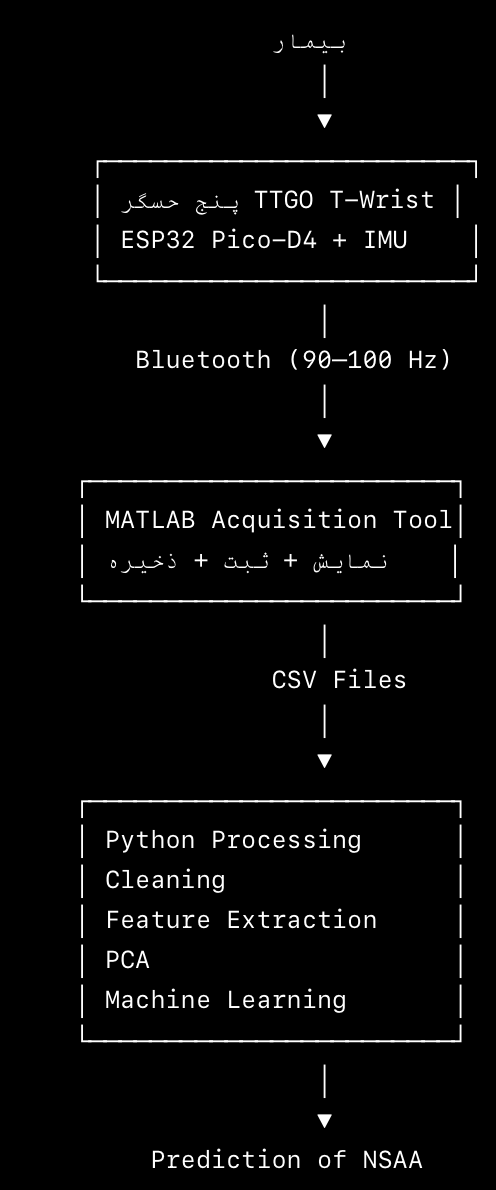
\includegraphics[width=0.2\linewidth]{Images/2_FlowChartSystemDesign}
	\caption{معماری کلی سامانه پیشنهادی و جریان داده از مرحله ثبت اطلاعات تا پیش‌بینی نمره عملکردی}
	\label{fig:2flowchartsystemdesign}
\end{figure}


\subsection{پیاده‌سازی سامانه داده‌برداری}

\subsubsection{چیدمان سامانه اندازه‌گیری}

اولین گام عملی در اجرای این پژوهش، طراحی سامانه داده‌برداری و تعیین نحوه استقرار حسگرها بر روی بدن آزمودنی بود. هدف از این مرحله، ثبت هم‌زمان حرکات اندام‌های مختلف بدن در هنگام اجرای آزمون‌های عملکردی و ایجاد مجموعه‌داده‌ای مناسب برای مراحل بعدی پردازش و تحلیل بود.

از آنجا که فعالیت‌های انتخاب‌شده در مقیاس \lr{NSAA} مجموعه‌ای از حرکات اندام فوقانی، اندام تحتانی و تغییرات وضعیت بدن را شامل می‌شوند، لازم بود چیدمان حسگرها به گونه‌ای انتخاب شود که اطلاعات کافی از حرکت بخش‌های مختلف بدن در اختیار قرار گیرد. در عین حال، افزایش تعداد حسگرها موجب پیچیده‌تر شدن فرآیند نصب، افزایش زمان آماده‌سازی بیمار و کاهش راحتی استفاده از سامانه می‌شد. بنابراین، در طراحی سامانه تلاش شد تعادلی میان میزان اطلاعات قابل ثبت و سادگی استفاده برقرار شود.

بر همین اساس، از پنج واحد حسگر پوشیدنی استفاده شد. یک حسگر بر روی پیشانی جهت ثبت حرکات سر، دو حسگر بر روی مچ دست راست و چپ و دو حسگر دیگر بر روی مچ پای راست و چپ نصب شدند. این چیدمان امکان ثبت هم‌زمان حرکات اندام‌های فوقانی و تحتانی را فراهم کرده و اطلاعات مناسبی از الگوی کلی حرکت بیمار در طول اجرای فعالیت‌های مختلف در اختیار قرار می‌دهد.

در این پژوهش از بردهای
 \lr{TTGO T-Wristband}
 به عنوان گره‌های حسگری استفاده شد. هسته پردازشی این بردها تراشه
 \lr{ESP32 Pico-D4}
   بوده و هر واحد به یک حسگر اینرسیایی مجهز است که قادر به اندازه‌گیری شتاب خطی و سرعت زاویه‌ای در سه محور می‌باشد. استفاده از این بردها علاوه بر ابعاد کوچک و قابلیت نصب آسان، امکان برقراری ارتباط بی‌سیم با رایانه را نیز فراهم می‌کرد.

داده‌های هر پنج حسگر به صورت هم‌زمان و از طریق ارتباط بلوتوث به رایانه منتقل شدند. نرخ نمونه‌برداری سامانه در حدود ۹۰ تا ۱۰۰ هرتز تنظیم شد که برای ثبت حرکات عملکردی بیماران و استخراج ویژگی‌های مورد نیاز در مراحل بعدی پژوهش مناسب ارزیابی شد.

\begin{figure}[H]
	\centering
	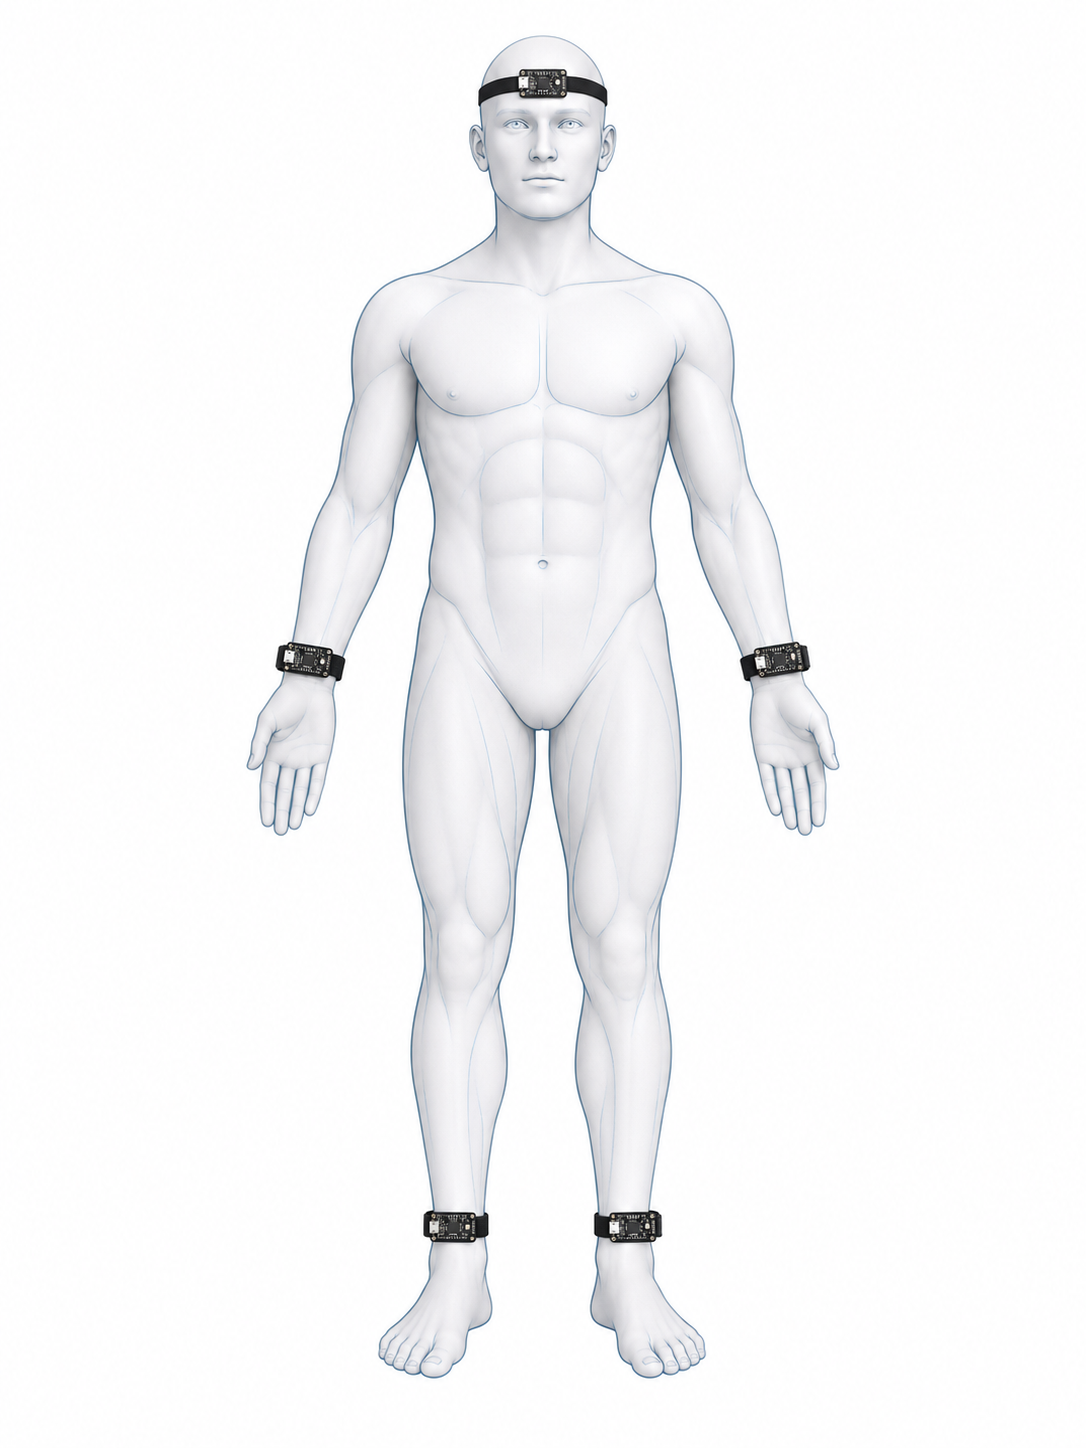
\includegraphics[width=0.3\linewidth]{Images/3_SensorsPlacement}
	\caption{محل نصب پنج حسگر اینرسیایی بر روی بدن آزمودنی}
	\label{fig:3sensorsplacement}
\end{figure}

\begin{table}[H]
	\centering
	\caption{مشخصات سامانه داده‌برداری}
	\label{tab:hardware}
	
	\begin{tabular}{ll}
		\toprule
		مشخصه & مقدار\\
		\midrule
		تعداد حسگرها & 5\\
		نوع برد & \lr{TTGO T-Wrist}\\
		پردازنده & \lr{ESP32 Pico-D4}\\
		نوع ارتباط & \lr{Bluetooth}\\
		نرخ نمونه‌برداری & 90 تا 100 هرتز\\
		سیگنال‌های ثبت‌شده & شتاب خطی و سرعت زاویه‌ای سه‌محوره\\
		\bottomrule
	\end{tabular}
	
\end{table}


\subsubsection{دلایل انتخاب چیدمان حسگرها}

یکی از تصمیم‌های مهم در طراحی سامانه، تعیین تعداد حسگرها و محل نصب آن‌ها بر روی بدن آزمودنی بود. هدف از این مرحله تنها ثبت بیشترین حجم داده ممکن نبود، بلکه دستیابی به چیدمانی بود که ضمن فراهم کردن اطلاعات کافی از الگوی حرکت بیمار، فرآیند نصب و استفاده از سامانه را نیز تا حد امکان ساده نگه دارد.

در صورتی که تعداد حسگرها بیش از حد افزایش یابد، علاوه بر افزایش زمان آماده‌سازی بیمار، احتمال جابه‌جایی حسگرها، ایجاد محدودیت در انجام حرکات و کاهش راحتی استفاده از سامانه نیز افزایش خواهد یافت. از سوی دیگر، استفاده از تعداد بسیار کم حسگرها ممکن است باعث از دست رفتن بخشی از اطلاعات حرکتی مورد نیاز شود. به همین دلیل، تلاش شد تعادل مناسبی میان پیچیدگی سامانه و اطلاعات قابل استخراج برقرار شود.

در این پژوهش، یک حسگر بر روی پیشانی نصب شد تا تغییرات وضعیت و حرکات سر در طول انجام آزمون‌ها ثبت شود. حرکات سر در بسیاری از فعالیت‌های عملکردی می‌تواند بیانگر استفاده از الگوهای جبرانی برای حفظ تعادل یا انتقال وزن باشد و در نتیجه اطلاعات مکملی از نحوه اجرای حرکت در اختیار قرار دهد.

دو حسگر دیگر بر روی مچ دست راست و چپ قرار گرفتند. اگرچه بسیاری از فعالیت‌های انتخاب‌شده در مقیاس \lr{NSAA} بر عملکرد اندام‌های تحتانی تمرکز دارند، اما در بخش قابل توجهی از این فعالیت‌ها، بیماران برای حفظ تعادل یا جبران ضعف عضلانی از اندام‌های فوقانی نیز استفاده می‌کنند. ثبت حرکات دست‌ها امکان بررسی این الگوهای جبرانی را فراهم می‌کند.

همچنین دو حسگر بر روی مچ پای راست و چپ نصب شدند تا اطلاعات مربوط به حرکات اندام‌های تحتانی، شامل تغییرات شتاب و سرعت زاویه‌ای پاها، در طول اجرای آزمون‌ها ثبت شود. از آنجا که اکثر فعالیت‌های عملکردی انتخاب‌شده مبتنی بر راه رفتن، برخاستن، نشستن، حفظ تعادل و سایر حرکات وابسته به اندام تحتانی هستند، داده‌های ثبت‌شده توسط این دو حسگر نقش اصلی را در تحلیل عملکرد بیماران ایفا می‌کنند.

در مجموع، چیدمان انتخاب‌شده امکان ثبت هم‌زمان حرکات سر، اندام‌های فوقانی و اندام‌های تحتانی را فراهم کرده و در عین حال، سامانه را به اندازه کافی ساده، سبک و قابل استفاده در محیط‌های درمانی نگه می‌دارد.


\subsubsection{نرم‌افزار تعبیه‌شده روی بردهای حسگر}

پس از طراحی چیدمان سامانه، لازم بود هر یک از واحدهای حسگری بتوانند داده‌های اندازه‌گیری‌شده را به صورت پیوسته دریافت و برای رایانه ارسال کنند. به همین منظور، برای تمامی بردهای مورد استفاده برنامه‌ای در محیط \lr{Arduino} توسعه داده شد که وظیفه راه‌اندازی حسگر، نمونه‌برداری از داده‌ها و ارسال آن‌ها از طریق ارتباط بی‌سیم را بر عهده داشت.

هر یک از پنج برد به صورت مستقل اجرا شده و پس از روشن شدن، ابتدا ارتباط با حسگر اینرسیایی را برقرار می‌کرد. پس از انجام مقداردهی اولیه، فرآیند نمونه‌برداری آغاز شده و داده‌های شتاب خطی و سرعت زاویه‌ای در سه محور به صورت پیوسته از حسگر دریافت می‌شدند.

استفاده از ساختار یکسان برای تمامی بردها موجب شد توسعه و نگهداری نرم‌افزار ساده‌تر شده و در صورت نیاز بتوان هر حسگر را بدون اعمال تغییر در سایر بخش‌های سامانه جایگزین کرد.


برای انتقال اطلاعات از ارتباط بلوتوث استفاده شد. هر برد به عنوان یک گره مستقل عمل کرده و داده‌های خود را به صورت جداگانه برای رایانه ارسال می‌کرد. به این ترتیب، نرم‌افزار توسعه‌یافته در محیط
 \lr{MATLAB}
  قادر بود اطلاعات هر پنج حسگر را به طور هم‌زمان دریافت و ذخیره کند.

در طراحی برنامه تلاش شد فرآیند ارسال داده‌ها با حداقل تأخیر انجام شود تا اختلاف زمانی میان داده‌های حسگرهای مختلف تا حد امکان کاهش یابد. همچنین قالب ارسال داده‌ها برای تمامی بردها یکسان در نظر گرفته شد تا فرآیند دریافت و ذخیره‌سازی اطلاعات در نرم‌افزار رایانه ساده‌تر شود.

خروجی هر بسته ارسالی شامل شناسه حسگر، زمان ثبت نمونه و مقادیر شتاب و سرعت زاویه‌ای در سه محور بود. استفاده از قالب یکسان برای تمامی حسگرها موجب شد داده‌های ثبت‌شده در مراحل بعدی پردازش به سادگی با یکدیگر همگام‌سازی و تحلیل شوند.

\begin{figure}[H]
	\centering
	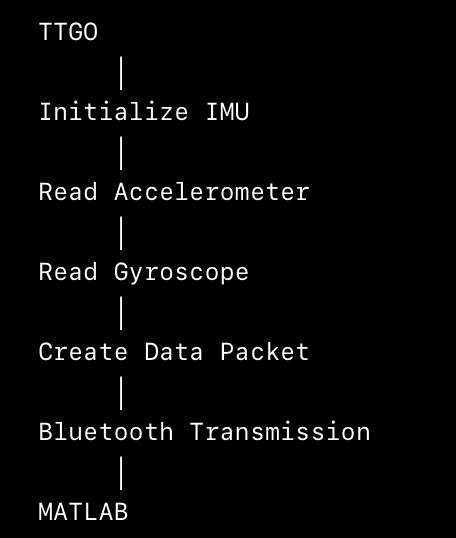
\includegraphics[width=0.3\linewidth]{Images/4_ArduinoCode}
	\caption{فلوچارت عملکرد نرم‌افزار اجراشده روی هر واحد حسگر}
	\label{fig:4arduinocode}
\end{figure}


\subsubsection{نرم‌افزار توسعه‌یافته در محیط \lr{MATLAB}}

پس از طراحی سامانه سخت‌افزاری، نیاز به نرم‌افزاری وجود داشت که بتواند داده‌های ارسال‌شده از حسگرها را به صورت هم‌زمان دریافت، نمایش و ذخیره‌سازی کند. به همین منظور، یک نرم‌افزار اختصاصی در محیط \lr{MATLAB} توسعه داده شد که به عنوان واسط میان سامانه اندازه‌گیری و مراحل بعدی پردازش داده عمل می‌کند.

در طراحی این نرم‌افزار تلاش شد تمامی نیازهای فرآیند داده‌برداری در یک محیط واحد فراهم شود تا اپراتور بدون نیاز به استفاده از نرم‌افزارهای جانبی بتواند کل فرآیند ثبت اطلاعات را مدیریت کند. به همین دلیل، امکاناتی مانند برقراری ارتباط با حسگرها، مشاهده وضعیت اتصال، نمایش داده‌های دریافتی، مدیریت اطلاعات آزمودنی و ذخیره‌سازی داده‌ها در قالب یک رابط کاربری یکپارچه پیاده‌سازی شد.

در ابتدای هر جلسه داده‌برداری، نرم‌افزار ارتباط بلوتوث با پنج حسگر را برقرار کرده و پس از اطمینان از اتصال صحیح تمامی واحدها، آماده دریافت داده می‌شود. اطلاعات ارسالی از هر حسگر به صورت مستقل دریافت شده و ضمن نمایش برخط، در حافظه نیز ذخیره می‌شوند تا در پایان هر آزمون فایل مربوطه ایجاد شود.

یکی دیگر از قابلیت‌های نرم‌افزار، مدیریت اطلاعات آزمودنی‌ها بود. پیش از شروع ثبت هر آزمون، مشخصات مربوط به بیمار، نوع فعالیت، شماره تکرار آزمون و سایر اطلاعات مورد نیاز توسط اپراتور وارد می‌شد. این اطلاعات همراه با داده‌های حسگر ذخیره شده و از ایجاد ابهام در مراحل بعدی پردازش جلوگیری می‌کرد.

به منظور کاهش احتمال خطا در فرآیند داده‌برداری، رابط کاربری نرم‌افزار به گونه‌ای طراحی شد که وضعیت ارتباط هر حسگر، شروع و پایان ثبت داده و وضعیت ذخیره‌سازی فایل‌ها به صورت واضح برای کاربر قابل مشاهده باشد. همچنین پس از پایان هر آزمون، داده‌های ثبت‌شده به صورت خودکار در مسیر مشخصی ذخیره می‌شدند تا ساختار منظمی از مجموعه داده‌های پروژه ایجاد شود.

با توجه به تعداد زیاد آزمون‌های انجام‌شده در طول پروژه، وجود چنین نرم‌افزاری نقش مهمی در افزایش سرعت داده‌برداری، کاهش خطاهای انسانی و یکپارچگی داده‌های ثبت‌شده ایفا کرد و بستری مناسب برای انجام مراحل بعدی پردازش و تحلیل اطلاعات فراهم ساخت.

\begin{figure}[H]
	\centering
	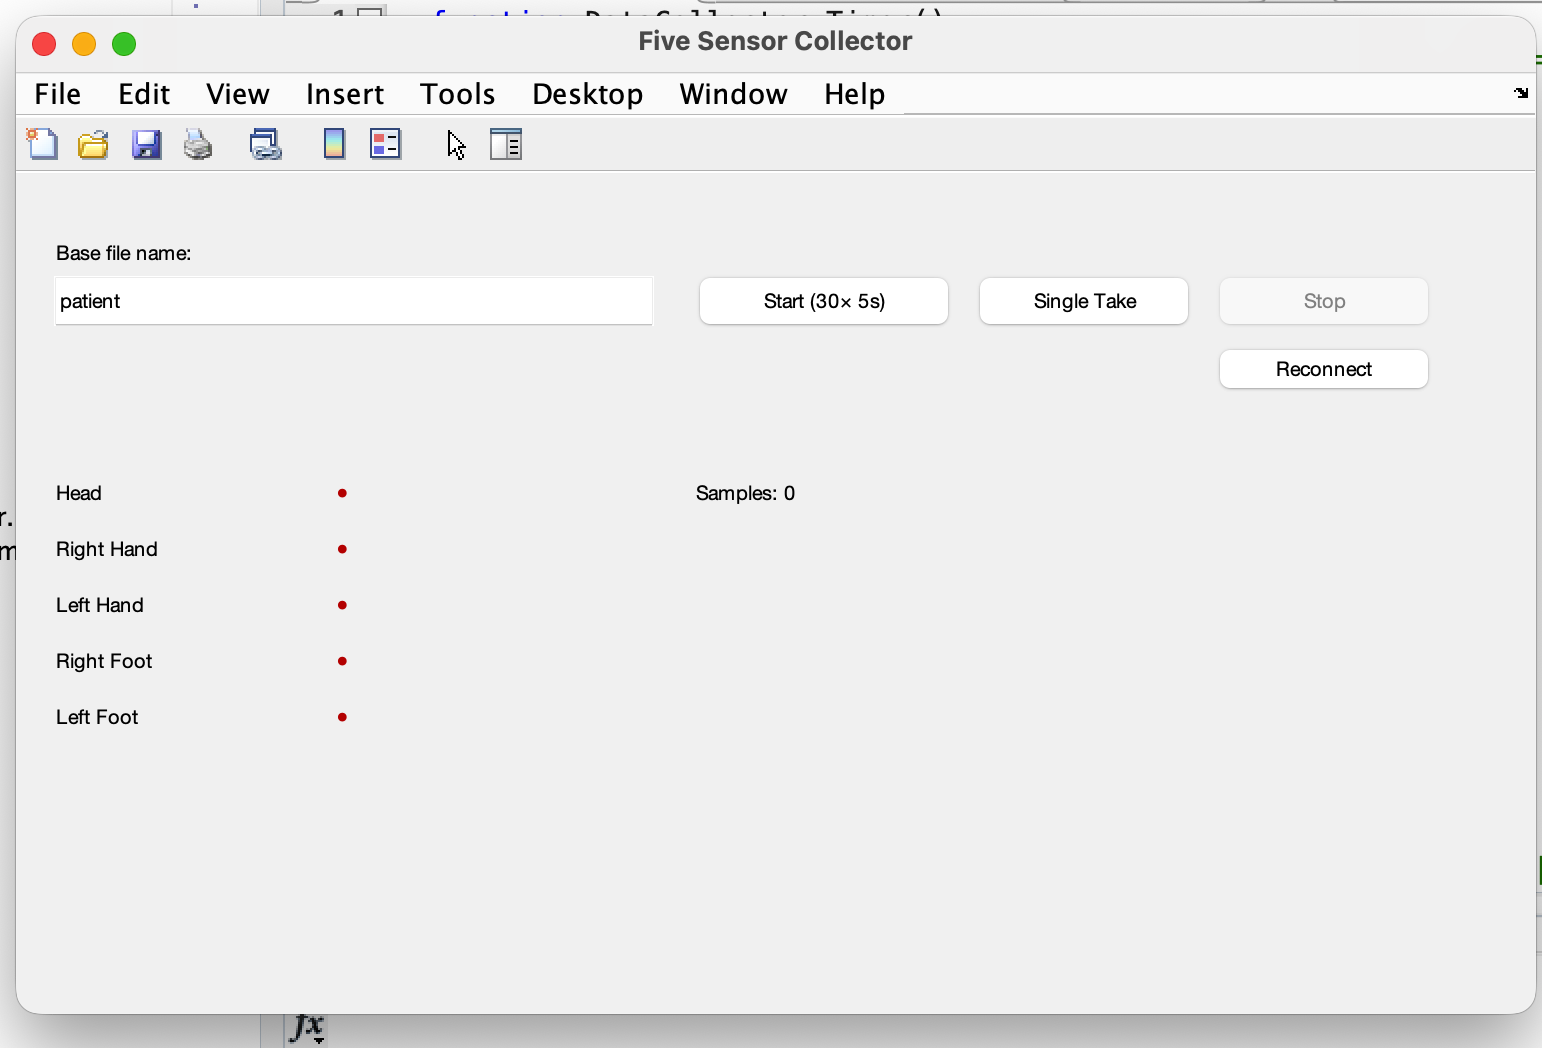
\includegraphics[width=0.7\linewidth]{Images/5_MatlabDataCollector}
	\caption{رابط کاربری نرم‌افزار توسعه‌یافته در محیط \lr{MATLAB} برای دریافت و ذخیره‌سازی هم‌زمان داده‌های حسگرها}
	\label{fig:5matlabdatacollector}
\end{figure}


\subsubsection{فرآیند انجام آزمون‌ها و ثبت داده‌ها}

پس از آماده‌سازی سامانه سخت‌افزاری و نرم‌افزار دریافت داده، فرآیند ثبت اطلاعات آزمودنی‌ها مطابق یک روال ثابت انجام می‌شد تا تمامی آزمون‌ها تحت شرایط یکسان ثبت شوند. یکسان بودن شرایط ثبت داده‌ها اهمیت زیادی داشت، زیرا هرگونه تغییر در نحوه نصب حسگرها یا اجرای آزمون‌ها می‌توانست بر کیفیت داده‌های جمع‌آوری‌شده و عملکرد مدل‌های یادگیری ماشین در مراحل بعدی تأثیر بگذارد.

در ابتدای هر جلسه، حسگرهای اینرسیایی مطابق چیدمان معرفی‌شده در بخش قبل بر روی پیشانی، مچ دو دست و مچ دو پا نصب می‌شدند. پس از روشن شدن تمامی بردها، ارتباط بلوتوث میان حسگرها و نرم‌افزار \lr{MATLAB} برقرار شده و وضعیت اتصال هر پنج حسگر بررسی می‌شد. پس از اطمینان از عملکرد صحیح سامانه، اطلاعات مربوط به آزمودنی و نوع آزمون در نرم‌افزار ثبت می‌شد.

در ادامه، بیمار فعالیت مورد نظر را مطابق دستور پزشک یا درمانگر اجرا می‌کرد. هم‌زمان با اجرای حرکت، داده‌های شتاب و سرعت زاویه‌ای هر پنج حسگر به صورت پیوسته ثبت و در رایانه ذخیره می‌شدند. ثبت اطلاعات از لحظه آغاز فعالیت تا پایان اجرای حرکت ادامه داشت و هیچ‌گونه پردازش یا فیلترگذاری در این مرحله بر روی داده‌های خام انجام نمی‌شد تا تمامی اطلاعات اولیه برای مراحل بعدی حفظ شوند.

پس از پایان هر آزمون، فایل مربوط به آن به صورت مجزا ذخیره شده و فرآیند برای فعالیت بعدی تکرار می‌شد. این روش باعث شد برای هر اجرای مستقل، یک فایل خام شامل اطلاعات تمامی حسگرها در اختیار باشد و در مراحل بعدی بتوان هر فعالیت را به صورت جداگانه مورد بررسی قرار داد.

در طول فرآیند داده‌برداری، تلاش شد تمامی آزمون‌ها تا حد امکان تحت شرایط مشابه انجام شوند. محل نصب حسگرها، نحوه قرارگیری آن‌ها روی بدن و ترتیب اجرای فعالیت‌ها در تمامی جلسات ثابت نگه داشته شد تا تغییرات مشاهده‌شده در داده‌ها تا حد امکان ناشی از عملکرد حرکتی آزمودنی باشد، نه تغییر در شرایط اندازه‌گیری.

به منظور کاهش تأثیر عوامل محیطی، تمامی آزمون‌ها توسط تیم درمانی و مطابق دستورالعمل یکسان انجام شدند و اپراتور در تمامی جلسات از روال ثابتی برای نصب حسگرها و ثبت اطلاعات استفاده کرد.


\begin{figure}[H]
	\centering
	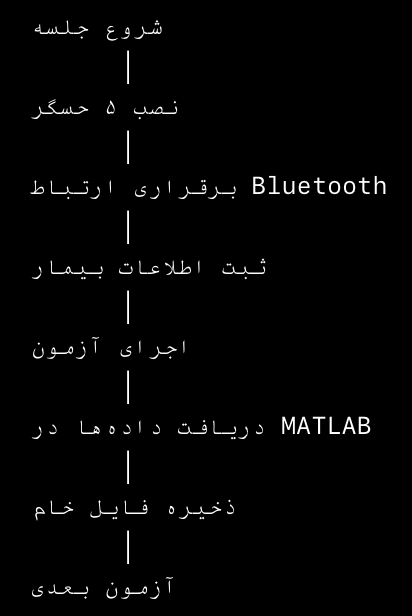
\includegraphics[width=0.3\linewidth]{Images/6_FlowChartDataCollecting}
	\caption{مراحل انجام فرآیند داده‌برداری در پژوهش حاضر}
	\label{fig:6flowchartdatacollecting}
\end{figure}


\subsection{پیش‌پردازش داده‌ها}

پس از پایان فرآیند داده‌برداری، فایل‌های خام ثبت‌شده مستقیماً برای آموزش مدل‌های یادگیری ماشین قابل استفاده نبودند. داده‌های خام علاوه بر آنکه شامل نویزهای ناشی از اندازه‌گیری بودند، بازه‌های زمانی قبل و بعد از اجرای هر فعالیت را نیز در بر می‌گرفتند و ساختار مناسبی برای استخراج ویژگی نداشتند. بنابراین پیش از ورود داده‌ها به مرحله یادگیری ماشین، مجموعه‌ای از عملیات پیش‌پردازش بر روی تمامی فایل‌ها انجام شد.

فرآیند پیش‌پردازش به گونه‌ای طراحی شد که تمامی داده‌ها با روشی یکسان پردازش شوند و امکان تکرار این مراحل برای داده‌های جدید نیز وجود داشته باشد. این فرآیند شامل فیلترگذاری سیگنال‌ها، جداسازی بازه زمانی مربوط به هر فعالیت، آماده‌سازی فایل‌ها، استخراج ویژگی‌ها، نرمال‌سازی داده‌ها و در صورت نیاز کاهش بعد داده‌ها بود.

مراحل مختلف این فرآیند در ادامه این فصل به ترتیب اجرای آن‌ها تشریح شده‌اند.


\subsubsection{دریافت فایل‌های خام}

در پایان هر آزمون، نرم‌افزار توسعه‌یافته در محیط 
\lr{MATLAB}
 داده‌های دریافتی از پنج حسگر را به صورت هم‌زمان در قالب فایل‌های جداگانه ذخیره می‌کرد. هر فایل شامل اطلاعات کامل یک اجرای مستقل از یک فعالیت مشخص بود و تمامی نمونه‌های ثبت‌شده از حسگرهای نصب‌شده روی بدن آزمودنی را در بر می‌گرفت.

از آنجا که هدف اصلی این مرحله حفظ تمامی اطلاعات اندازه‌گیری‌شده بود، هیچ‌گونه پردازش یا تغییر بر روی داده‌ها هنگام ذخیره‌سازی انجام نشد و تمامی سیگنال‌ها به صورت خام ثبت شدند. این موضوع باعث شد در مراحل بعدی امکان اعمال روش‌های مختلف پردازش سیگنال بدون از دست رفتن اطلاعات اولیه وجود داشته باشد.

پس از پایان جلسات داده‌برداری، تمامی فایل‌های خام به عنوان ورودی مرحله پیش‌پردازش مورد استفاده قرار گرفتند.


\subsubsection{فیلترگذاری سیگنال‌ها}

سیگنال‌های ثبت‌شده توسط حسگرهای اینرسیایی علاوه بر اطلاعات حرکتی، شامل نویزهای ناشی از اندازه‌گیری، ارتعاشات محیطی و خطاهای لحظه‌ای حسگر نیز بودند. به منظور کاهش تأثیر این عوامل، پیش از هرگونه تحلیل، عملیات فیلترگذاری بر روی تمامی داده‌ها انجام شد.

در این پژوهش از فیلتر پایین‌گذر باترورث مرتبه چهارم استفاده شد. این فیلتر به دلیل پاسخ فرکانسی مناسب و حفظ شکل اصلی سیگنال، یکی از متداول‌ترین روش‌های مورد استفاده در پردازش داده‌های بیومکانیکی محسوب می‌شود.

اعمال این فیلتر موجب حذف بخش عمده نویزهای فرکانس بالا شده و سیگنال‌های نرم‌تر و مناسب‌تری را برای مراحل بعدی پردازش فراهم کرد.

در این پژوهش، برای تمامی سیگنال‌های ثبت‌شده از فیلتر پایین‌گذر 
\lr{Butterworth}
 مرتبه چهار استفاده شد. اعمال فیلتر پیش از سایر مراحل پردازش باعث شد مؤلفه‌های نویزی حذف شده و سیگنال‌های حاصل، نمایانگر دقیق‌تری از حرکت واقعی آزمودنی باشند. تمامی مراحل فیلترگذاری به صورت خودکار بر روی تمامی فایل‌های ثبت‌شده انجام شدند.


\subsubsection{جداسازی فعالیت‌ها}

در برخی از آزمون‌ها، داده‌های ثبت‌شده علاوه بر بخش اصلی حرکت، شامل زمان قبل از شروع و پس از پایان فعالیت نیز بودند. وجود این قسمت‌ها می‌توانست موجب استخراج ویژگی‌های نامرتبط و کاهش دقت مدل‌های یادگیری ماشین شود.

به همین دلیل، پس از فیلترگذاری، بازه زمانی مربوط به اجرای واقعی هر فعالیت از سیگنال جدا شد. در فعالیت‌هایی که نیاز به جداسازی داشتند، با استفاده از الگوریتم تشخیص حرکت توسعه‌یافته در محیط
 \lr{MATLAB}،
  ابتدا زمان شروع و پایان فعالیت تعیین و سپس تنها بخش مربوط به اجرای حرکت استخراج شد.

در برخی فعالیت‌ها که کل فایل تنها شامل اجرای همان حرکت بود، نیازی به انجام این مرحله وجود نداشت و داده‌ها مستقیماً وارد مراحل بعدی شدند.


\subsubsection{آماده‌سازی داده‌ها برای تحلیل}

پس از پایان مراحل فیلترگذاری و جداسازی فعالیت‌ها، داده‌های آماده‌شده برای ورود به محیط 
\lr{Python}
 ذخیره شدند. در این مرحله، تمامی فایل‌ها دارای ساختاری یکنواخت بودند و هر نمونه تنها شامل اطلاعات مربوط به اجرای یک فعالیت مشخص بود.

در ادامه، اسکریپت‌های توسعه‌یافته در محیط
 \lr{Python} 
 فایل‌های تولیدشده را خوانده و پس از بررسی کامل بودن داده‌ها، نمونه‌های نامعتبر یا ناقص را حذف کردند. همچنین قالب داده‌ها به گونه‌ای بازآرایی شد که تمامی نمونه‌ها با ساختاری یکسان وارد مرحله استخراج ویژگی شوند.

خروجی این مرحله مجموعه‌داده‌ای پاک‌سازی‌شده و استاندارد بود که مبنای استخراج ویژگی‌ها و آموزش مدل‌های یادگیری ماشین در مراحل بعدی پژوهش قرار گرفت.



\subsection{استخراج ویژگی‌ها}

پس از انجام مراحل پیش‌پردازش، سیگنال‌های ثبت‌شده توسط حسگرهای اینرسیایی برای استفاده مستقیم در الگوریتم‌های یادگیری ماشین مناسب نبودند. از آنجا که این الگوریتم‌ها معمولاً بر روی مجموعه‌ای از ویژگی‌های عددی آموزش داده می‌شوند، لازم بود اطلاعات موجود در سیگنال‌های خام به مجموعه‌ای از شاخص‌های کمی تبدیل شوند که بتوانند خصوصیات اصلی حرکت را توصیف کنند.

به همین منظور، در این پژوهش فرآیند استخراج ویژگی بر روی تمامی سیگنال‌های آماده‌شده انجام شد. در این مرحله، برای هر محور از شتاب‌سنج و ژیروسکوپ هر حسگر، مجموعه‌ای از ویژگی‌های آماری و سیگنالی محاسبه گردید. این ویژگی‌ها به گونه‌ای انتخاب شدند که بتوانند اطلاعاتی درباره شدت حرکت، میزان تغییرات، پراکندگی داده‌ها، تقارن سیگنال و سایر خصوصیات حرکتی را در اختیار مدل‌های یادگیری ماشین قرار دهند.

تمامی مراحل استخراج ویژگی به صورت خودکار و با استفاده از اسکریپت‌های توسعه‌یافته در محیط 
\lr{Python}
 انجام شد و برای تمامی نمونه‌ها فرآیندی یکسان اجرا گردید. خروجی این مرحله، ماتریسی از ویژگی‌ها بود که هر سطر آن متناظر با یک نمونه و هر ستون آن متناظر با یک ویژگی استخراج‌شده بود.


\subsubsection{ویژگی‌های استخراج‌شده}

برای هر یک از سیگنال‌های ثبت‌شده، مجموعه‌ای از ویژگی‌های حوزه زمان محاسبه شد. انتخاب این ویژگی‌ها بر اساس مطالعات پیشین در زمینه تحلیل حرکت و همچنین قابلیت آن‌ها در توصیف رفتار آماری سیگنال انجام گرفت.

ویژگی‌های استخراج‌شده شامل شاخص‌هایی نظیر مقدار میانگین، انحراف معیار، واریانس، حداقل و حداکثر مقدار، دامنه تغییرات، میانه، چارک‌های اول و سوم، فاصله بین چارکی، انرژی سیگنال، مقدار
 \lr{RMS}
 \footnote{\lr{Root Mean Square}}
، چولگی، کشیدگی، ضریب تغییرات، میانگین قدر مطلق، میانگین تغییرات متوالی و سایر ویژگی‌های آماری بودند.

از آنجا که هر حسگر شامل شش کانال اندازه‌گیری (سه محور شتاب‌سنج و سه محور ژیروسکوپ) است، تمامی ویژگی‌ها برای هر یک از این کانال‌ها به صورت مستقل محاسبه شدند. در نهایت، ویژگی‌های استخراج‌شده از تمامی حسگرها با یکدیگر ادغام شده و بردار ویژگی نهایی هر نمونه تشکیل گردید.


	\begin{table}[H]
		\centering
		\caption{ویژگی‌های استخراج‌شده از هر سیگنال}
		\begin{LTR}
			\begin{tabular}{ll}
				\toprule
				ویژگی & توضیح\\
				\midrule
				\lr{Count} & تعداد نمونه‌ها\\
				\lr{Mean} & میانگین\\
				\lr{Standard Deviation} & انحراف معیار\\
				\lr{Variance} & واریانس\\
				\lr{Minimum} & کمینه\\
				\lr{Maximum} & بیشینه\\
				\lr{Range} & دامنه تغییرات\\
				\lr{Median} & میانه\\
				\lr{First Quartile} & چارک اول\\
				\lr{Third Quartile} & چارک سوم\\
				\lr{Interquartile Range} & فاصله بین چارک‌ها\\
				\lr{Mean Absolute Value} & میانگین قدر مطلق\\
				  \lr{ Root Mean Square} & RMS\\
				\lr{Skewness} & چولگی\\
				\lr{Kurtosis} & کشیدگی\\
				\lr{Energy} & انرژی\\
				\lr{Entropy} & آنتروپی\\
				\lr{Zero Crossing Rate} & نرخ عبور از صفر\\
				\bottomrule
			\end{tabular}
		\end{LTR}
	\end{table}

از آنجا که پنج حسگر مورد استفاده قرار گرفتند و هر حسگر شامل شش سیگنال (سه محور شتاب و سه محور سرعت زاویه‌ای) بود، ویژگی‌های فوق برای تمامی کانال‌ها استخراج شدند. در نتیجه، برای هر آزمون یک بردار ویژگی با ابعاد بالا تولید شد که مبنای مراحل بعدی تحلیل قرار گرفت.

در پایان فرآیند استخراج ویژگی، برای هر نمونه تعداد 690 ویژگی عددی تولید شد. این مجموعه ویژگی‌ها به عنوان ورودی مدل‌های یادگیری ماشین مورد استفاده قرار گرفت.


\begin{figure}[H]
	\centering
	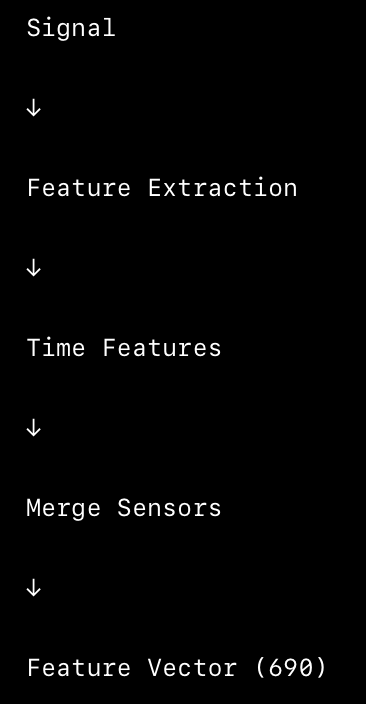
\includegraphics[width=0.3\linewidth]{Images/7_FlowChartFeatureExtraction}
	\caption{استخراج ویژگی}
	\label{fig:7flowchartfeatureextraction}
\end{figure}


\subsection{کاهش بعد ویژگی‌ها}

پس از استخراج ویژگی‌ها، برای هر نمونه یک بردار شامل 690 ویژگی در اختیار قرار گرفت. اگرچه استفاده از تعداد زیاد ویژگی‌ها می‌تواند اطلاعات بیشتری از داده‌ها در اختیار مدل قرار دهد، اما افزایش ابعاد داده ممکن است موجب افزایش پیچیدگی محاسبات، ایجاد هم‌بستگی میان ویژگی‌ها و کاهش توان تعمیم مدل شود. به همین دلیل، در این پژوهش تأثیر استفاده از روش کاهش بعد نیز مورد بررسی قرار گرفت.

برای این منظور، از روش تحلیل مؤلفه‌های اصلی 
\footnote{\lr{Principal Component Analysis (PCA)}}
 استفاده شد. این روش با تبدیل ویژگی‌های اولیه به مجموعه‌ای از مؤلفه‌های متعامد، بیشترین میزان واریانس داده را در تعداد کمتری از متغیرها حفظ می‌کند.

پیش از اعمال
 \lr{PCA}،
 تمامی ویژگی‌ها با استفاده از روش استاندارد سازی،
 \footnote{\lr{Standardization}}
   نرمال‌سازی شدند تا میانگین هر ویژگی برابر صفر و انحراف معیار آن برابر یک شود. انجام این مرحله از آن جهت ضروری است که 
 \lr{PCA}
    نسبت به مقیاس ویژگی‌ها حساس بوده و وجود اختلاف زیاد میان دامنه مقادیر ویژگی‌ها می‌تواند بر نتایج تحلیل مؤلفه‌های اصلی تأثیر بگذارد.

در این پژوهش دو رویکرد مستقل مورد بررسی قرار گرفت. در رویکرد اول، مدل‌های یادگیری ماشین مستقیماً بر روی ویژگی‌های استخراج‌شده آموزش داده شدند. در رویکرد دوم، 
 \lr{PCA}
 به عنوان بخشی از 
 \lr{Pipeline}
  تعریف شد و تنها بر روی داده‌های آموزش برازش داده شد و سپس مدل‌های یادگیری ماشین با استفاده از ویژگی‌های کاهش‌یافته آموزش داده شدند. مقایسه نتایج این دو رویکرد امکان بررسی تأثیر کاهش بعد بر عملکرد مدل‌ها را فراهم کرد.


\subsection{آموزش مدل‌های یادگیری ماشین}

پس از استخراج ویژگی‌ها و آماده‌سازی مجموعه‌داده، مرحله آموزش مدل‌های یادگیری ماشین آغاز شد. هدف از این مرحله، بررسی توانایی الگوریتم‌های مختلف در پیش‌بینی نمره عملکردی بیماران بر اساس ویژگی‌های استخراج‌شده از داده‌های حسگرهای اینرسیایی بود.

به منظور انجام یک مقایسه منصفانه، تمامی مدل‌ها با استفاده از مجموعه ویژگی‌های یکسان آموزش داده شدند و معیارهای ارزیابی نیز برای تمامی آن‌ها به صورت مشابه محاسبه گردید. همچنین، تمامی مراحل پیش‌پردازش مورد نیاز هر مدل، شامل نرمال‌سازی ویژگی‌ها و در صورت استفاده، کاهش بعد با روش 
 \lr{PCA}،
 در قالب یک
 \lr{Pipeline}
  یکپارچه پیاده‌سازی شد تا از بروز نشت اطلاعات
 \footnote{\lr{Data Leakage}}
    بین داده‌های آموزش و آزمون جلوگیری شود.

در این پژوهش، دو روش مختلف برای تقسیم داده‌ها و ارزیابی مدل‌ها مورد بررسی قرار گرفت که در ادامه معرفی می‌شوند.


\subsubsection{تقسیم‌بندی تصادفی با تعداد نمونه ثابت}

در نخستین روش ارزیابی، برای هر کلاس تعداد ثابتی از نمونه‌ها به صورت تصادفی برای آموزش و آزمون انتخاب شدند. در هر تکرار، 20 نمونه از هر کلاس برای آموزش و 5 نمونه برای آزمون مورد استفاده قرار گرفتند. این فرآیند به صورت تصادفی 100 بار تکرار شد تا اثر انتخاب تصادفی داده‌ها بر عملکرد مدل‌ها کاهش یابد.

در پایان، میانگین معیارهای ارزیابی در تمامی تکرارها به عنوان عملکرد نهایی هر مدل گزارش شد. این روش امکان بررسی پایداری مدل‌ها در برابر تقسیم‌بندی‌های مختلف داده را فراهم می‌کند.


\subsubsection{اعتبارسنجی متقاطع}

در کنار تقسیم‌بندی تصادفی، از روش اعتبارسنجی متقاطع طبقه‌بندی‌شده نیز برای ارزیابی مدل‌ها استفاده شد. در این روش، داده‌ها با استفاده از الگوریتم
 \lr{Stratified K-Fold}
 به پنج بخش تقسیم شدند؛ به گونه‌ای که نسبت نمونه‌های هر کلاس در تمامی دسته‌ها حفظ شود.

به منظور کاهش وابستگی نتایج به یک تقسیم‌بندی خاص، فرآیند اعتبارسنجی پنج‌تایی پنج مرتبه با چینش‌های تصادفی مختلف تکرار شد. بنابراین عملکرد هر مدل بر اساس نتایج حاصل از 25 مرحله آموزش و آزمون محاسبه گردید.

استفاده از اعتبارسنجی متقاطع باعث می‌شود تمامی نمونه‌های موجود در مجموعه‌داده حداقل یک بار در مجموعه آزمون قرار گیرند و در نتیجه برآورد دقیق‌تری از توانایی تعمیم مدل به دست آید.



\subsubsection{مدل‌های مورد استفاده}

به منظور بررسی عملکرد روش‌های مختلف یادگیری ماشین، سه الگوریتم متداول برای مسئله طبقه‌بندی انتخاب شدند. این مدل‌ها شامل ماشین بردار پشتیبان 
 \footnote{\lr{SVM}}،
 نزدیک‌ترین همسایه 
 \footnote{\lr{KNN}}
  و جنگل تصادفی
 \footnote{\lr{Random Forest}}
    بودند.

مدل ماشین بردار پشتیبان با استفاده از هسته شعاعی
 \footnote{\lr{RBF Kernel}}
  پیاده‌سازی شد. این الگوریتم به دلیل توانایی مناسب در مدل‌سازی مرزهای تصمیم‌گیری غیرخطی، یکی از پرکاربردترین روش‌ها در مسائل طبقه‌بندی داده‌های زیستی محسوب می‌شود.

الگوریتم
 \lr{KNN}
  نیز با استفاده از پنج همسایه نزدیک اجرا شد. این روش بر اساس شباهت میان نمونه‌های آموزشی و نمونه جدید تصمیم‌گیری می‌کند و به عنوان یکی از ساده‌ترین روش‌های یادگیری نظارت‌شده شناخته می‌شود.

همچنین، الگوریتم
 \lr{Random Forest}
  با 500 درخت تصمیم آموزش داده شد. استفاده از تعداد زیاد درخت‌ها موجب افزایش پایداری مدل و کاهش احتمال بیش‌برازش نسبت به یک درخت تصمیم منفرد می‌شود.



\subsubsection{\lr{Pipeline} پردازش داده}

به منظور جلوگیری از نشت اطلاعات بین مجموعه آموزش و آزمون، تمامی مراحل پیش‌پردازش در قالب یک
 \lr{Pipeline}
  پیاده‌سازی شدند. در این ساختار، ابتدا ویژگی‌ها با استفاده از روش
 \lr{StandardScaler}
    استانداردسازی شدند. سپس در صورت فعال بودن کاهش بعد، تحلیل مؤلفه‌های اصلی
 (\lr{PCA})
      تنها بر روی داده‌های آموزش برازش داده شد و همان تبدیل بر روی داده‌های آزمون اعمال گردید. در نهایت، داده‌های پردازش‌شده برای آموزش مدل یادگیری ماشین مورد استفاده قرار گرفتند.

استفاده از 
 \lr{Pipeline}
باعث شد تمامی مراحل پردازش در هر بار آموزش مدل به صورت مستقل انجام شوند و احتمال بروز
 \lr{Data Leakage}
 به طور کامل حذف گردد.



\subsection{معیارهای ارزیابی}

به منظور مقایسه عملکرد مدل‌های مختلف، از چندین معیار متداول ارزیابی طبقه‌بندی استفاده شد. این معیارها دید مناسبی از توانایی مدل در تشخیص صحیح کلاس‌ها ارائه می‌کنند.

در این پژوهش، معیارهای
 \lr{Accuracy}، \lr{Precision}، \lr{Recall}، \lr{F1-score}
  و
\lr{Specificity}
 برای تمامی مدل‌ها محاسبه شدند. همچنین، به منظور بررسی نحوه توزیع خطاهای مدل، ماتریس درهم‌ریختگی
  (\lr{Confusion Matrix})
 نیز برای هر الگوریتم استخراج شد.

برای مسائل چندکلاسه، مقادیر
 \lr{Precision}، \lr{Recall} و \lr{F1-score}
  با استفاده از میانگین
 \lr{Macro}
    محاسبه شدند تا تمامی کلاس‌ها سهم یکسانی در ارزیابی عملکرد مدل داشته باشند. همچنین، مقدار 
 \lr{Specificity}
     نیز بر اساس میانگین اختصاصی هر کلاس محاسبه گردید.


\subsection{روند اجرای آزمایش‌ها}

پس از آماده‌سازی مجموعه‌داده و پیاده‌سازی مدل‌های یادگیری ماشین، مجموعه‌ای از آزمایش‌ها برای ارزیابی عملکرد مدل‌ها طراحی و اجرا شد. هدف از این آزمایش‌ها، بررسی تأثیر روش‌های مختلف کاهش بعد و مقایسه عملکرد الگوریتم‌های یادگیری ماشین در پیش‌بینی نمرات عملکردی بیماران بود.

به همین منظور، تمامی آزمایش‌ها در دو حالت مستقل انجام شدند. در حالت اول، مدل‌های یادگیری ماشین مستقیماً با استفاده از ویژگی‌های استخراج‌شده آموزش داده شدند. در حالت دوم، پیش از آموزش مدل‌ها، روش تحلیل مؤلفه‌های اصلی
\lr{(PCA)}
 بر روی داده‌های آموزش اعمال شد و سپس مدل‌ها با استفاده از ویژگی‌های کاهش‌یافته آموزش دیدند.

برای هر یک از این دو حالت، دو روش مختلف ارزیابی شامل تقسیم‌بندی تصادفی داده‌ها و اعتبارسنجی متقاطع مورد استفاده قرار گرفت. تمامی آزمایش‌ها برای تمامی الگوریتم‌های یادگیری ماشین با تنظیمات یکسان اجرا شدند تا امکان مقایسه منصفانه نتایج فراهم شود.

در پایان هر آزمایش، معیارهای ارزیابی محاسبه و نتایج حاصل برای تحلیل نهایی ذخیره شدند. این نتایج در فصل بعد مورد بررسی و مقایسه قرار خواهند گرفت.


\subsubsection{مراحل اجرای \lr{Pipeline}}

روند اجرای هر آزمایش مطابق مراحل زیر انجام شد:

\begin{enumerate}
	\item بارگذاری داده‌های پیش‌پردازش‌شده؛
	
	\item تقسیم داده‌ها به مجموعه آموزش و آزمون؛
	
	\item استانداردسازی ویژگی‌ها با استفاده از \lr{StandardScaler}؛
	
	\item اعمال \lr{PCA} (در صورت فعال بودن) تنها بر روی داده‌های آموزش؛
	
	\item آموزش مدل یادگیری ماشین؛
	
	\item پیش‌بینی برچسب نمونه‌های آزمون؛
	
	\item محاسبه معیارهای ارزیابی و ذخیره نتایج.
\end{enumerate}



\begin{figure}[H]
	\centering
	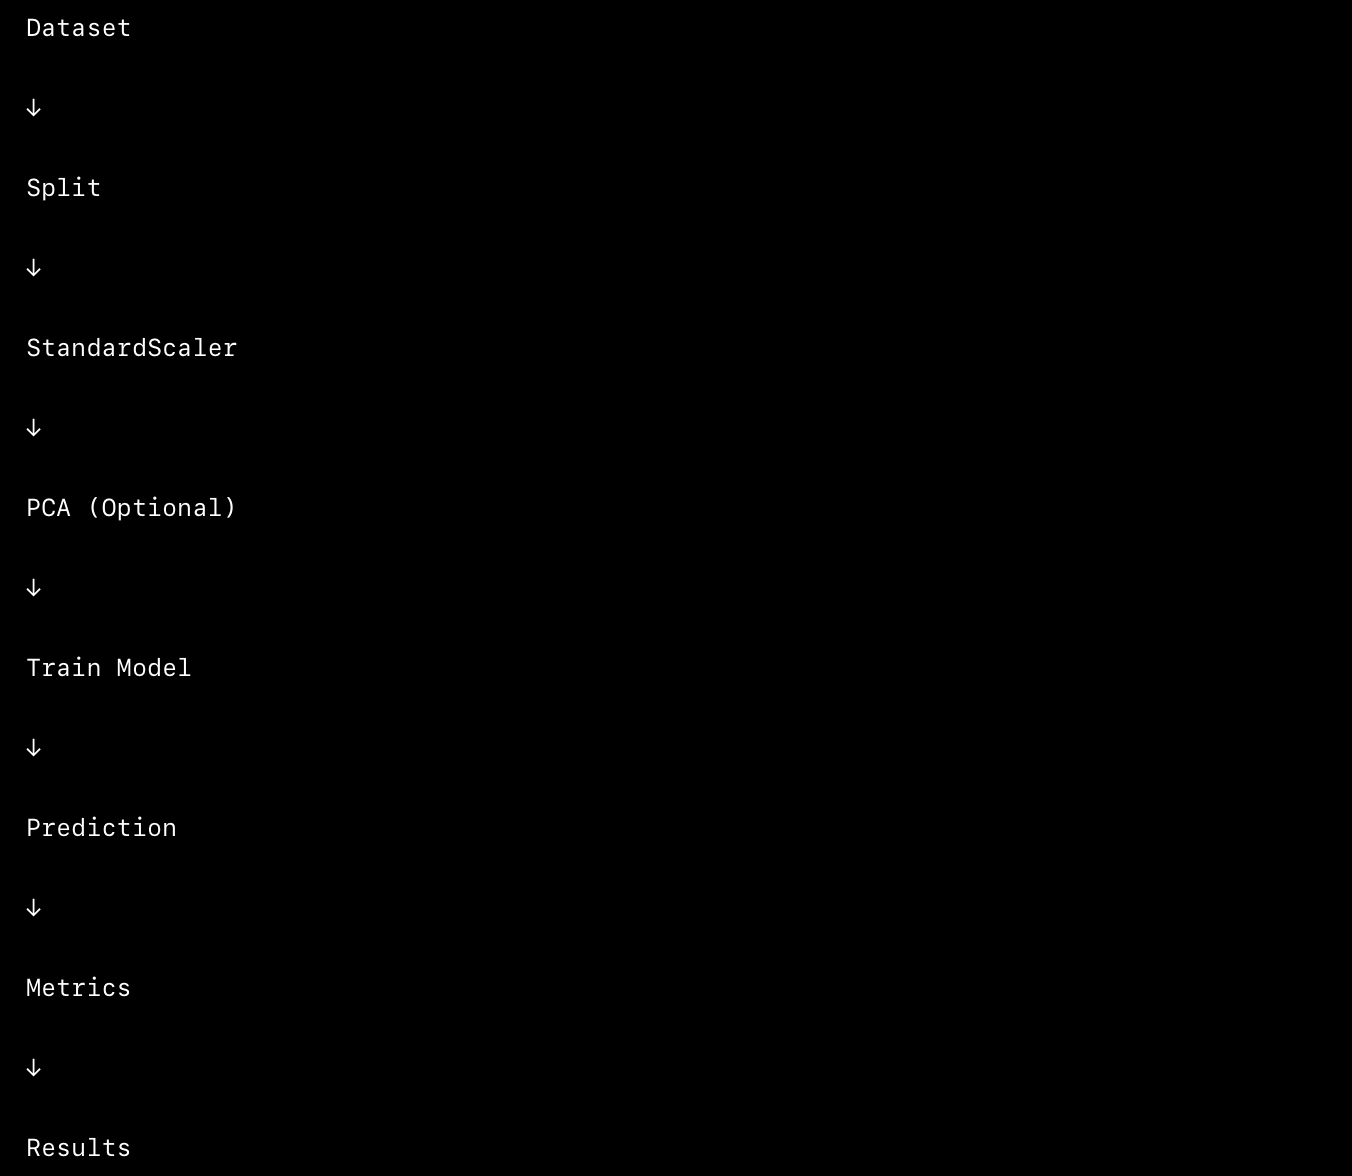
\includegraphics[width=0.5\linewidth]{Images/8_FlowChartPipline}
	\caption{روند اجرای هر آزمایش در \lr{Pipeline} طراحی‌شده}
	\label{fig:8flowchartpipline}
\end{figure}


\subsection{ابزارهای نرم‌افزاری مورد استفاده}

در این پژوهش، توسعه بخش‌های مختلف سامانه با استفاده از چند محیط نرم‌افزاری انجام شد.

برنامه‌های اجراشده روی بردهای حسگر با استفاده از محیط 
\lr{Arduino IDE}
 توسعه یافتند. دریافت داده‌ها، مدیریت ارتباط بلوتوث و ذخیره‌سازی اطلاعات در محیط 
\lr{ MATLAB}
  انجام شد. همچنین تمامی مراحل پیش‌پردازش، استخراج ویژگی، کاهش بعد و آموزش مدل‌های یادگیری ماشین در محیط
\lr{Python}
    پیاده‌سازی گردید.

در بخش یادگیری ماشین از کتابخانه‌های
 \lr{NumPy}، \lr{Pandas}، \lr{Scikit-learn} 
 و 
 \lr{Matplotlib}
  برای پردازش داده‌ها، آموزش مدل‌ها و تحلیل نتایج استفاده شد.


\section*{جمع‌بندی}

در این فصل، مراحل طراحی و پیاده‌سازی سامانه پیشنهادی به طور کامل تشریح شد. ابتدا ساختار سامانه داده‌برداری، چیدمان حسگرهای اینرسیایی و نرم‌افزارهای توسعه‌یافته برای ثبت اطلاعات معرفی شدند. سپس فرآیند پیش‌پردازش داده‌ها، استخراج ویژگی، کاهش بعد و آموزش مدل‌های یادگیری ماشین توضیح داده شد.

در ادامه، نحوه طراحی آزمایش‌ها، روش‌های ارزیابی مدل‌ها و معیارهای مورد استفاده برای سنجش عملکرد الگوریتم‌ها ارائه گردید. بر اساس این زیرساخت، در فصل بعد نتایج حاصل از اجرای مدل‌های مختلف ارائه شده و عملکرد آن‌ها با یکدیگر مقایسه خواهد شد.
